\chapter{Einleitung}
Continuous Integration, kurz CI, ist ein Entwicklungsverfahren, welches Entwickler dazu drängt mehrmals am Tag bei einem gemeinsamen Repository beizutragen. Jeder Beitrag wird automatisch verifiziert. Dieser Vorgang erlaubt es dem Team Probleme früh zu erkennen.
Durch einen regelmäßigen Beitrag der Entwickler können Fehler schnell erkannt und lokalisiert werden.

\begin{figure}[!htb]
	\centerline{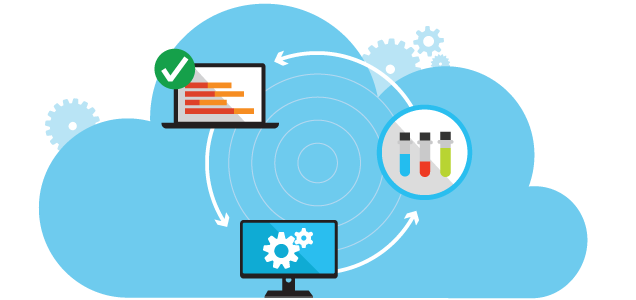
\includegraphics[width=0.5\textwidth]{img/ci}}
	\caption{Continuous Integration Kreislauf \cite{continuous-integration-circle}.}
	\label{ci}
\end{figure}

\section{Spät Änderungen integrieren}
Ein spät erkannter Fehler führt zu einer schwereren Eingrenzung des Codebereiches. Durch einen regelmäßigen Beitrag zum Code und den damit verbunden automatischen Überprüfungen sind Fehler direkt mit zeitlich kleineren Arbeitseinheiten verknüpft. Dadurch können sie schneller gefunden werden.

\begin{quote}
“Continuous Integration doesn’t get rid of bugs, but it does make them dramatically easier to find and remove.” - Martin Fowler, Chief Scientist, ThoughtWorks \cite{continuous-integration-thoughtworks}
\end{quote}

\section{Kosten}
Eine ständige Entwicklung mit verbundener Integration und Testphase ist teuer. Denken Sie hier langfristiger. Der angesprochene Zeitfaktor zum Finden ist kritisch. Früh erkannte Fehler sind einfach zu beheben und verbrauchen somit weniger Ressourcen. Wird nicht nach dem Entwicklungsverfahren gelebt entstehen längere Zeitperioden in dem eine Integration statt findet. Eine solche Zeitspanne bedeutet eine exponentielle Steigerung der nötigen Ressourcen zum Finden und Beheben der Fehler. Sie fahren demnach deutlich besser, wenn Fehler möglichst früh erkannt und behoben werden.

\section{Projektstabilität}
Spät erkannte Fehler rauben Ressourcen, welche an anderer Stelle wichtig sind. Werden Mitarbeiter von der Entwicklung zur Fehlerbehebung geschoben ist der Zeitplan in Gefahr. Im schlimmsten Fall können Kritische Fehler das komplette Projekt zum Fall bringen. Mit CI sollten diese Gefahren in akzeptablen Größen auftauchen. Fehlerbehebungen sind gut zu planen und bringen nicht überraschend das Projekt in Gefahr. 

\section{Vorteile}
Jedes Entwicklungsunternehmen profitiert von vielen Vorteilen gegenüber einer späten Integration dank CI.
\begin{itemize}
	\item Die langen intensiven Integrationen entfallen
	\item Ein häufiger Beitrag erhöht die Sichtbarkeit der Codeänderungen für andere Mitarbeiter und fördert somit die Kommunikation
	\item  Probleme werden schnell erfasst und behoben
	\item Es kann mehr Zeit in die eigentliche Entwicklung anstatt in die Fehlerbehebung investiert werden
	\item Aufbauende Änderungen basieren auf einem festen Fundament
	\item Direktes Feedback über Funktionsfähigkeit des neuen Codes
	\item Eine Reduzierung von Integrationsproblemen erlaubt eine häufigere Auslieferung der Software
\end{itemize}